%% LaTeX template for BSc Computing for Games final year project dissertations
%% by Edward Powley
%% Games Academy, Falmouth University, UK

%% Based on:
%% bare_jrnl.tex
%% V1.4b
%% 2015/08/26
%% by Michael Shell
%% see http://www.michaelshell.org/
%% for current contact information.
%%
%% This is a skeleton file demonstrating the use of IEEEtran.cls
%% (requires IEEEtran.cls version 1.8b or later) with an IEEE
%% journal paper.
%%
%% Support sites:
%% http://www.michaelshell.org/tex/ieeetran/
%% http://www.ctan.org/pkg/ieeetran
%% and
%% http://www.ieee.org/

%%*************************************************************************
%% Legal Notice:
%% This code is offered as-is without any warranty either expressed or
%% implied; without even the implied warranty of MERCHANTABILITY or
%% FITNESS FOR A PARTICULAR PURPOSE! 
%% User assumes all risk.
%% In no event shall the IEEE or any contributor to this code be liable for
%% any damages or losses, including, but not limited to, incidental,
%% consequential, or any other damages, resulting from the use or misuse
%% of any information contained here.
%%
%% All comments are the opinions of their respective authors and are not
%% necessarily endorsed by the IEEE.
%%
%% This work is distributed under the LaTeX Project Public License (LPPL)
%% ( http://www.latex-project.org/ ) version 1.3, and may be freely used,
%% distributed and modified. A copy of the LPPL, version 1.3, is included
%% in the base LaTeX documentation of all distributions of LaTeX released
%% 2003/12/01 or later.
%% Retain all contribution notices and credits.
%% ** Modified files should be clearly indicated as such, including  **
%% ** renaming them and changing author support contact information. **
%%*************************************************************************


\documentclass[journal]{IEEEtran}

\usepackage{graphicx}
% Insert additional usepackage commands here

\begin{document}
%
% paper title
% Titles are generally capitalized except for words such as a, an, and, as,
% at, but, by, for, in, nor, of, on, or, the, to and up, which are usually
% not capitalized unless they are the first or last word of the title.
% Linebreaks \\ can be used within to get better formatting as desired.
% Do not put math or special symbols in the title.
\title{Does Exploration Behaviour That is Based of Human-Like Curiosity Perceive AI Smartness?}
%
%
% author name
\author{Tomas Mazurkevic}

% The paper headers -- please do not change these, but uncomment one of them as appropriate
% Uncomment this one for COMP320
\markboth{COMP320: Research Review and Proposal}{COMP320: Research Review and Proposal}
% Uncomment this one for COMP360
% \markboth{COMP360: Dissertation}{COMP360: Dissertation}

% make the title area
\maketitle

% As a general rule, do not put math, special symbols or citations
% in the abstract or keywords.
\begin{abstract}
Abstract not written yet, as you may see. But as a side note - bullet points 
\end{abstract}

\section{Introduction}
% The very first letter is a 2 line initial drop letter followed
% by the rest of the first word in caps.
% 
% form to use if the first word consists of a single letter:
% \IEEEPARstart{A}{demo} file is ....
% 
% form to use if you need the single drop letter followed by
% normal text (unknown if ever used by the IEEE):
% \IEEEPARstart{A}{}demo file is ....
% 
% Some journals put the first two words in caps:
% \IEEEPARstart{T}{his demo} file is ....
% 
% Here we have the typical use of a "T" for an initial drop letter
% and "HIS" in caps to complete the first word.
\IEEEPARstart{T}{hroughout} the last 30 years researchers are trying to create clever artificial intelligence (AI) using different methods and algorithms. Recent achievements in such area really worthy of respect. For example, AlphaGo being able to beat world champions in Go \cite{alphago} or OpenAI playing Atari games and, in most of them, getting higher scores than human players \cite{mnih2015human}. AI in games, however, is used to create non-player characters (NPCs), which can have very different pattern varying from AI as Adversary to AI as Spectacle \cite{treanor2015ai}. 

AI in video games is very crucial when it's used as one of the main mechanics. Intelligent non-player characters (NPCs) are extremely hard to make due to the nature of it's complexity. The more complex it is the more outcomes developers will have to consider and the more problems will occur during development \cite{gdchalo2}. Moreover, it tends to use lots of computer's resources \cite{gdchalo2}, such as memory, poor run-time, scalability and other, which brings more challenges.

Some of the very complex algorithms, such as reinforcement learning (RL), deep Q-learning, curiosity-driven, evolution-based and a lot more are being used in video games as testbeds for different disciplines that vary from training algorithms \cite{aiinvideogames}\cite{robotplayground} to robotics \cite{schmidhuber2006developmental}\cite{colledanchise2018behavior}\cite{brady1985artificial}\cite{oudeyer2004intelligent} to Go \cite{schaul2011measuring}\cite{alphago}. However, due to specificity of games, it is not always the best solution. Depending on game's design, simple methods or less complex ones can be used instead of previously mentioned algorithms. As an example, Finite State Machine (FSM) became a common one to use after the success of the game F.E.A.R with only using three states \cite{orkin2006three} or Monte Carlo Tree Search (MTCS) \cite{chaslot2008monte}, which has been used in creation of a new paradigm for Go \cite{gelly2011monte}\cite{gelly2012grand}. 

A more simple yet very effective technique for AI creation is behaviour tree (BT). It has first been introduced in \cite{gdchalo2} and is now commonly being used in different game engines such as Unreal Engine, which is what this project is going to use. It is believed, that BTs are ``highly modular, flexible and reusable" \cite{colledanchise2017behavior}. (ADD MORE HERE WITH FIGURES OF BEHAVIOUR TREE SAMPLES)

\section{Related Work} %~134
The main focus of this paper is to demonstrate a potentially valuable AI behaviour that is not complex yet efficient in enhancing smart AI. In section different AI implementation methods will be discussed, both complex and simple as well as why and how AI is used both in games and real life. This will include human's curiosity and discuss it from psychological view, why it's one of the main factor towards human's willingness to learn and gain new knowledge and some relevant learning algorithm implementations to make interesting and smart AI. Turing's Test will also be included in this section, which will describe it's use, advantages and disadvantages and why it's used as a testing method for this project. Moreover, it will describe how smartness is going to be measured in this context. Methodology and hypotheses will be reviewed in sections III and IV respectively. Methodology will also include research artefact, introduce to what the participants will be asked to do and how data will be collected. The proposed behaviour implementation will be handled in Unreal Engine 4 (UE4) using our team's game for easier testing purpose as there will be enough assets to create a unique world which AI could be tested on.
\begin{itemize}
	\item Explain the main focus of this paper
	\item Explain the testing subject I'm gonna use
	\item Briefly explain next sections
	\item Will be using my third year team project game to test the implementation on.
\end{itemize}

\subsection{AI Importance in Games}
Different methods that are used in AI learning - reinforcement, evolution-based, q-learning, curiosity-driven, etc. 
\begin{itemize}
	\item Why is it complex and important?
	\item What does it help to achieve? 
	\item Talk about Halo 2 AI (and maybe TF2 bots - research more)
	\item Talk about how simple implementations can be much more efficient than complex learning methods
\end{itemize}

Artificial intelligence has a big place in the modern world. Robots are being created to ease human's life, machines that can beat best players in the world in most complex games such as Go \cite{alphago} or chess. But AI for games is not created to overcome player's abilities. It's there to enhance player's experience, to make the game more engaging and fun to play \cite{aiinvideogames} while acting realistically \cite{chaslot2008monte}. Therefore, other difficult problems are being solved, which may not fit well with AI used in real life, but they are still very valuable. Solving AI problems using games has become pretty common nowadays and is used for many areas as a testing purpose \cite{schaul2011measuring}. The testbeds can alter from simplicity to diversity \cite{schaul2011measuring} and can include testing natural language understanding and/or production, theorem proving, physical and simulated robotics and the original Turing's test \cite{schaul2011measuring}.

AI for games is mainly developed to increase player's engagement and/or satisfaction feelings \cite{halo2}. Whether that's bosses or companions, friends or enemies. Given the flexibility of AI, games use it very differently. Thus, some games decide to enhance players' positive emotions and some might make the game feel terrifying. It is designers' aspiration to create such feelings depending on the game itself. The satisfaction from defeating extremely hard bosses you spent hours on is unforgettable as well as the fright from the ever building up atmosphere enhanced by terrifying creatures. All of this makes games unique and entertaining for people whose desire is to rest from our real world.

Of course, not every game must have AI, but what's the most frustrating a game can have is experience ruining AI. In which case, immersion breaks and players start complaining about game being "unplayable" even though it's only enemies or friends behaving inappropriately or silly. Indeed, when players want to have a relaxing time playing a game, which is broken by AI only is upsetting. This again shows how important AI is for games, which requires considerable amount of effort put into to create fun and engaging experience. So, to prove this point, next couple subsections (or paragraphs) will present and discuss successful use of AI creating both positive and negative emotions.

\subsubsection{Alien: Isolation}
Artificial intelligence is very commonly used to create various feelings alongside an atmosphere of the game. A good example of this is game called Alien: Isolation created by Creative Assembly, Feral Interactive and awarded a BAFTA Games Award for Audio Achievement. The alien enemy is the main threat that makes the player fear it to create a horrifying experience. However, atmosphere around it accompanied with audio also plays a huge role. Moreover, specifically in this game, the AI is very complex and smart. In fact, it has two personalities, in other words - brains \cite{seller2019horrific}. The first one playing the role of the Alien ``having perfect information about the environment" \cite{seller2019horrific} and the second one responsible for movement and immediate stimuli response \cite{seller2019horrific}. Indeed, this together creates a very interesting and exceptional behaviour of the AI. The alien reacts to any sudden movements, noises and other characters that are not player. In fact, there are other enemies besides aliens, which the alien itself is attacking. This creates different scenarios and entertaining gameplay where player can bait the alien to kill any hazard on the player's way that is another NPC.

\subsubsection{Halo 2}
Another excellent example of smart and flexible AI is Halo 2 developed by Bungie Studios, which used previously mentioned technique - behaviour trees \cite{behaviourtreeofhalo2}. AI in Halo 2 ``lives in a simulated world" \cite{halo2} - emphasizes Chris Butcher, one of four Engineering Leads at Bungie Studios, who was responsible for certain sections of Halo's development - and there's very small distinction between NPCs and the player \cite{halo2}. Although every creature in Halo 2 feels unique they all function the same. NPCs perceive the world using their "senses", interpret all this data and make decisions based on them \cite{halo2}. This is mostly the same capabilities human players have. Therefore, this makes AI feel very smart, fun to play against and, more importantly, feel like a real human player. In addition, players can witness AI characters getting surprised, making mistakes and questionable decisions \cite{halo2}, because they perceive their environment the same way a human player would. This particularly makes AI predictable, which was the aim of Halo 2 making NPCs consistent \cite{halo2} and is considered to be "smart" AI \cite{gamemakertoolkit}. Thus, players can predict NPCs' actions, but consequences will be unpredictable.

Even more impressive feature AI in Halo 2 has is their new joint behaviour system \cite{halo2}. It allows NPCs to communicate between each other and inform other allies of any threats or request a tactical move. This wouldn't be possible for players to notice if developers didn't add speech to it. Indeed, whenever an enemy does any action, it is followed by it saying it out loud. This is a simple if/then statement, but it improves AIs predictability, which therefore increases its smartness as was mentioned before. In fact, small features that don't exactly relate to AI implementation might also enhance the way it feels, making it smarter and unique.

AI importance in games
\begin{itemize}
	\item What makes AI important in games?
	\item What does it help to accomplish in games? Satisfaction, level of difficulty, engagement, relationship between the player and NPCs
	\item Has a big research area - making AI interesting and solving complex problems, which can be applied to real world problems with robots
	\item Potentially talk about Halo 2 AI, which made the game very engaging and fun to play - as an example
	\item Talk about what smart AI is like in games (video reference)
\end{itemize}

\subsection{Curiosity}
Curiosity is a driving force for human's exploration, which consists of exploration, investigation and learning behaviours \cite{wu2013curiosity}\cite{kashdan2004curiosity}. It makes people chase for knowledge and investigate anything new and potentially valuable. Moreover, curiosity is beneficial for people on two levels: the individual and the social \cite{kashdan2010curiosity}. The first one is represented as the "innate love of learning and of knowledge... without the lure of any profit" \cite{loewenstein1994psychology}. The social level, on the other hand, is presented as ``an ingredient for enhancing personal relationships'' \cite{wu2013curiosity}.

In computational form, curiosity can be split into different designs \cite{wu2013curiosity}. However, in this case, we are going to look at a curious exploratory agent. It can reach high learning effectiveness in an unknown environment \cite{wu2013curiosity}\cite{macedo2005role}. Even though the behaviour this project is going to test will be hard-coded, it gives opportunity for further learning, such as having learning algorithm like curiosity-driven instead of hard-coding. Moreover, due to curiosity being proposed as algorithmic principles \cite{wu2013curiosity}\cite{pang2009curiosity}\cite{karaoguz2011curiosity} it enhances machines' "exploration" and allows it to own ``the desire to improve the model network's knowledge about the world." \cite{schmidhuber1991possibility}. It also had success in unsupervised developmental robotics \cite{schmidhuber2006developmental}\cite{oudeyer2004intelligent}.

Curiosity-driven learning in games can show some fascinating results. In \cite{burda2018large}, researchers train AI using curiosity-driven learning without extrinsic rewards and test it on dozens of games, 48 of which are Atari games. Previously, this kind of learning was using either extrinsic or intrinsic reward system, however, this paper applies no rewards for AI and yet demonstrates positive results. The research has also been using Random Network Distillation (RND), which showed a significant progress in Montezuma's Revenge \cite{openairl}\cite{montezumarevenge}. It scored more than twice as high than average human player, which shows potential in future development. However, this kind of learning doesn't always score as high as in Montezuma's Revenge. This shows that it still requires improvements to be used in today's games and potentially in robotics.

The way curiosity-driven learning works is that the AI tries to predict the next frame (next-state prediction / noisy-tv problem - might not be suitable)
\begin{itemize}
	\item Why do curiosity?
	\item Examples of curiosity-driven behaviours
	\item How will it make AI look smarter?
	\item Challenges that occur trying to implement such behaviour
	\item Explain why curiosity is one of the main drivers that lead human to explore/do something
	\item What is smartness and how could it be measured?
\end{itemize}

\subsection{Turing's Test}
``Intelligence measures an agent’s ability to achieve goals in a wide range of
environments." \cite{legg2007universal}

``Intelligence is a very general mental capability that, among other things, involves
the ability to reason, plan, solve problems, think abstractly, comprehend complex
ideas, learn quickly and learn from experience." \cite{gottfredson1997mainstream}
\begin{itemize}
	\item Explain Turing's test
	\item Why use this testing method?
	\item Explain how I'm gonna test my implementation
	\item Briefly go over what question I'm going to use to get the participants' data
	\item Analyse critics regarding Turing's test and explain why I chose this method
\end{itemize}

\section{Hypotheses}
The aim of this project is to implement a simple exploration behaviour based of human's curiosity. Therefore, this project's first hypothesis is that exploration behaviour will perceive AI smartness compared to non-curious AI. The second hypothesis aims the participants to distinguish player's behaviour from AI's behaviour, which will be provided by the questionnaire data. After analysing this data, the results will show whether the curious behaviour is leaning towards human-like, which will prove or disprove this project's hypothesis.

These hypotheses are mainly aimed to see if exploration behaviour based on human's curiosity enhances smartness for AI in games. Due to AI in games primarily being used for NPCs and concentrated on combat systems, idle states are often excluded from having "smart" behaviour. This is done in order to save computer's resoruces for more important matter, such as combat. However, having a smart looking AI for walking simulators can therefore enhance player's experience in such genres. This could become a decisive factor for developers that want to create a gorgeous walking simulator using fantastic looking environment enhanced with smart and interesting artificial intelligence.
\begin{itemize}
	\item The AI will feel smarter
	\item The participants won't distinguish human's behaviour and AI (which is good)
\end{itemize}

\section{Methodology}
\begin{table}
	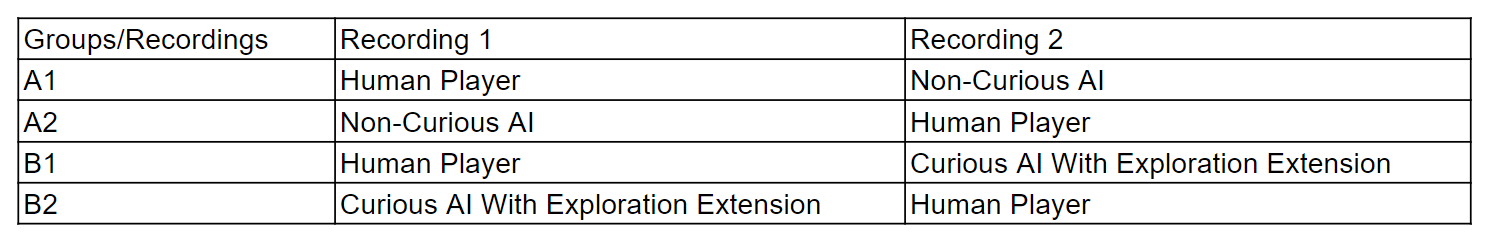
\includegraphics[width=\linewidth]{MethodologyTable.PNG}
	\caption{Methodology}
	\label{tab:methodology}
\end{table}
The testing of the hypotheses will be handled by separating participants into two groups randomly chosen and shown video recordings selected at random, see Table \ref{tab:methodology}. All of this will be done randomly to minimise bias towards either side as much as possible. The first group will be presented with non-curious AI behaviour and human player's behaviour or vice versa. The second group, on the other hand, will be introduced with curious AI behaviour, which was enhanced by exploration extension, and human player's behaviour or vice versa. 

\subsection{Research Artefact}
For the proposed hypotheses testing the project will be using our team project game that is made using Unreal Engine 4 (UE4) with a few changes in the game to represent first-person walking simulator. The environment in the game will also be changed in order to more accurately generate curiosity from both AI and player perspectives. Moreover, the exploration behaviour this paper is going to test will be implemented using Behaviour Tree. The behaviour will be thoroughly tested for any possibly experience ruining errors and playtested before the start of the research. Afterwards, it will be recorded and, during the testing process, data will be gathered from participants. Another AI behaviour will also be recorded before the data gathering as well as human's behaviour. All the recordings will be handled by the free recording software called Open Broadcaster Software (OBS) due to it's simplicity and quality of entries.

\begin{figure}
	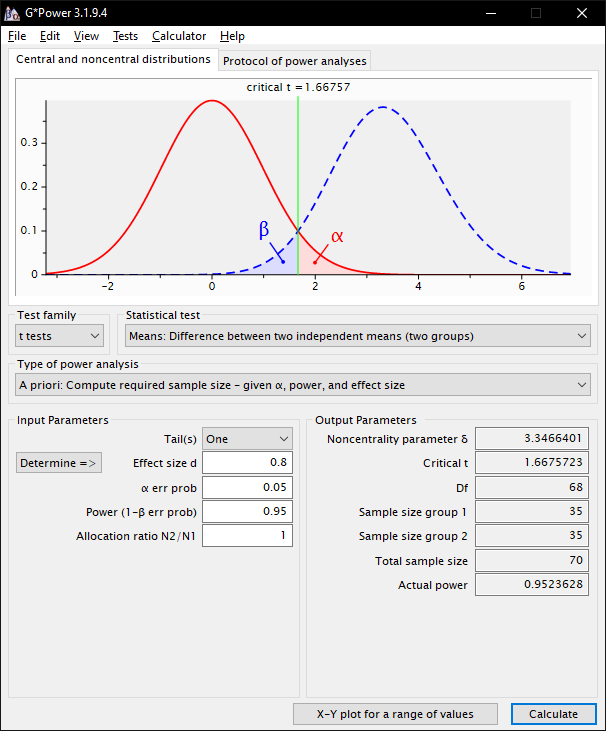
\includegraphics[width=\linewidth]{GPower.PNG}
	\caption{Screenshot of a-priori power analysis to calculate sample size using G*Power available at: http://www.gpower.hhu.de/}
	\label{fig:gpower}
\end{figure}

\subsection{Participants}
Due to the need of human player's behaviour, seven to eight people will be asked to play the game and record their gameplay. This necessity does not require a lot of participants and, moreover, they will not be taking part in providing research data and are not counted towards the required sample size presented in Figure \ref{fig:gpower}. Ideally, they will have no to little experience with such games to generate more curious nature of human. The goal for these participants will be to explore the game's environment. However, they will not be told that to avoid bias towards having unnatural curiosity behaviour, which could influence project's testing. Instead, they will have an ability to do whatever they desire. This will instead generate more natural behaviour and thought process from these participants and will benefit this project's outcome. It will be handled in the first place and all the people that will be recruited to record their gameplay will be given a consent form to sign due to university's ethics policy. Participants' data will be anonymous and will not be stored anywhere due to the fact that only game's view, in other words gameplay, will be recorded.

The participants that are going to take part in the research and answer the questionnaire will likely be from different disciplines both inside and outside of Games Academy due to bigger audience variety and experience in such field. These participants will be asked to sign an information sheet given to them before the start of the testing to inform about any necessary information and get a consent. There will be four groups of participants observing different recordings of human player and AI behaviours that are selected randomly. From the Figure \ref{fig:gpower}, it is shown that the project will need 70 participants given the effect size of 0.8, which is considered large by the Cohen's guidelines. However, if the project brings more attention, sample size could be increased accordingly, giving more data to analyse.

\subsection{Questionnaire}
After the participants have viewed the recordings, they will be asked to complete a survey. The survey will provide the necessary data to analyse and later discuss the efficiency of the proposed exploration behaviour enhancing the AI's smartness. First of all, the survey will ask how often the participant plays games and whether they have played any first-person walking simulators. This will give the understanding of participant's experience with games, which might influence their insight of the research. The second part of this survey consists only of one question asking which behaviour felt smarter in their opinion before getting the necessary data to analyse curiosity in each behaviour. The last part consists of measuring behaviours' curiosity level using a scale from one to seven and asking the participants whether they have distinguished an AI from human. In which case if the answer to this questions is positive, they will be asked to answer two more questions that include a short description of the distinguishable features AI had and how smart it felt on a scale of one to seven. This will give more detailed data to analyse regarding AI.

\begin{itemize}
	\item How the hypotheses will be tested?
	\item Include potential questions - explain what data each question will provide
	\item Maybe include an example of similar test?
	\item Include how smartness will be measured - If the simple behaviour's score is less than exploration behaviour, it will mean that the exploration behaviour is potentially making AI look smarter
\end{itemize}

\section{Conclusion}
So, in conclusion, artificial intelligence for games is vey important in todays games, however terminology "smart" is interpreted differently (THIS NEEDS TO BE INCLUDED IN TURING'S TEST). It is not about winning human player's all the time how it is to maintain game's fun and satisfaction levels. Moreover, games are also used as testbeds for AI, which can further improve real life robotics. Robots, however, are becoming more and more advanced hence making curiosity for robots more feasible. Even though curiosity is becoming more possible for robots there are still other major problems to be solved before it becomes real.

% references section

\bibliographystyle{IEEEtran}
\bibliography{References}

% Appendices

\appendices
\section{First appendix}
Appendices are optional. Delete or comment out this part if you do not need them.

% Unused
% This is essential because of the nature of some recordings to be likely of not providing the necessary curiosity for more accurate testing purpose (participants)
% Explain curiosity - human behaviour often depends on person's intentions to explore. Why apply to AI? The aim of this paper is not to create curiosity-driven AI in Unreal Engine 4 (UE4), but to implement and test a particular behaviour and see how people react. Whether they like it or not, whether they think it behaves smart and etc. The aim of this implementation is to find a small nuance that can make the AI feel and act smarter.
% Statechart-Based AI in Practice
% Monte-Carlo Tree Search: A New Framework for Game AI
% Building Human-Level AI for Real-Time Strategy Games

% that's all folks
\end{document}
